\section*{Sistemas con \(N> 2\) grados de libertad}


\item
\begin{minipage}[t][1.8cm]{0.65\textwidth}
\textbf{Molécula triatómica | Oscilaciones longitudinales}\\
Se esquematiza en la figura una molécula triatómica simétrica.
Entre dos átomos de masa $m$ hay uno de masa $M = 2 m$.
Se modelan los enlaces bajo el modelo de elasticidad de Hooke con constante $k$ y longitud natural $\ell_0$.
\end{minipage}
\begin{minipage}[c][0cm][t]{0.7\textwidth}
%   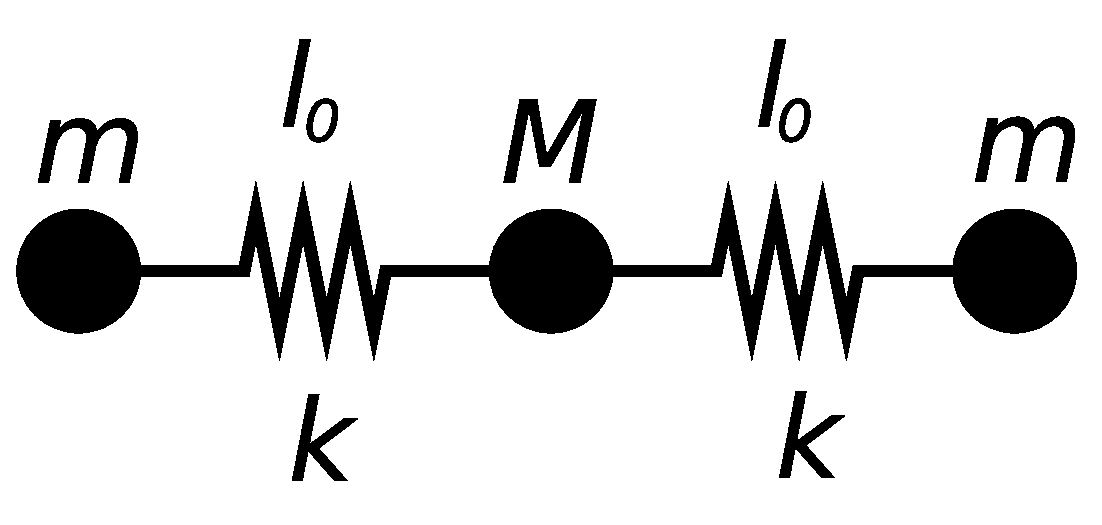
\includegraphics[width=\textwidth]{ej1-9}
	\begingroup
		% \tikzset{every picture/.style={scale=0.4}}%
		\input{\detokenize{figuras/ownCO2_tikz}}
	\endgroup
\end{minipage}
\begin{enumerate}
	\item Encuentre las ecuaciones para la dinámica de cada átomo en la dirección longitudinal a la molécula, \(\hat{x}\).
	Asuma que los átomos tienen impedido un movimiento transversal.
	\item Halle las frecuencias de los modos normales. 
	\item Dibuje las configuraciones de cada modo. 
	\item Si el centro de masa de la molécula se mueve con $\vec{v}_0 = \mathrm{cte}\, \hat{x}$, escriba la solución $\vec{x}(t)$.
	\item Determine las condiciones iniciales para excitar sólo el modo de mayor frecuencia.
\end{enumerate}



\item
% \begin{minipage}[t][2.2cm]{0.5\textwidth}
\textbf{Molécula triatómica | Oscilaciones transversales}\\
Analice las oscilaciones transversales para el sistema del problema anterior.
Para su mejor comprensión puede imaginarlo como el esquema de la figura, en el cual los átomos en los extremos pueden subir/bajar pero solidarios a unas imaginarias barras enhebradas a vástagos laterales. 
% \end{minipage}
% \begin{minipage}[c][0cm][t]{0.45\textwidth}
%   \includegraphics[width=\textwidth]{\detokenize{moléculaT}}
% \end{minipage}
\begin{figure}[h]
	\centering
	\input{figuras/tikzn2gl_2}
\end{figure} 
\begin{enumerate}
	\item Encuentre las ecuaciones de movimiento de los átomos.
	¿Qué diferencia hay en el caso con resortes \emph{slinky} y con $\ell_0 \neq 0$ en las ecuaciones de movimiento bajo la aproximación de pequeñas oscilaciones? 
	\item Halle las frecuencias de los modos normales.
	\item Dibuje la configuración correspondiente a cada modo normal.
	Determine los desplazamientos de cada átomo en función del tiempo (solución más general posible para cada átomo).
	\item ¿Qué condiciones iniciales permiten excitar sólo el segundo modo?
	\item Si se fuerza al átomo del centro con frecuencias incrementalmente mayores, ¿qué modos se van observando?
	\item Abstrayendonos de la idea de una molécula y pensando el sistema como compuesto de partículas y resortes, ¿cómo se modifican los resultados anteriores si la párticula en la derecha se enlaza, no a un vástago sino, a una pared a través de un resorte igual a los demás como muestra la siguiente figura?
	\begin{figure}[h]
		\centering
		\input{figuras/tikzn2gl_2_f}
		% \includegraphics[clip,scale=0.5]{\detokenize{moléculaT_fijo_libre}}
	\end{figure} 
\end{enumerate}



\item 
\begin{minipage}[t][1.2cm]{0.6\textwidth}
(*) \textbf{Tres partículas en red de resortes}\\
Considere el sistema de la figura, en la que los resortes verticales tienen longitud natural $l_0$ y constante $k_1$, y los horizontales $a_0= 0$ (son ``slinkies'') y $k_2$.
Calcule las frecuencias propias y los modos normales. 
\end{minipage}
\begin{minipage}[c][1.2cm][t]{0.35\textwidth}
  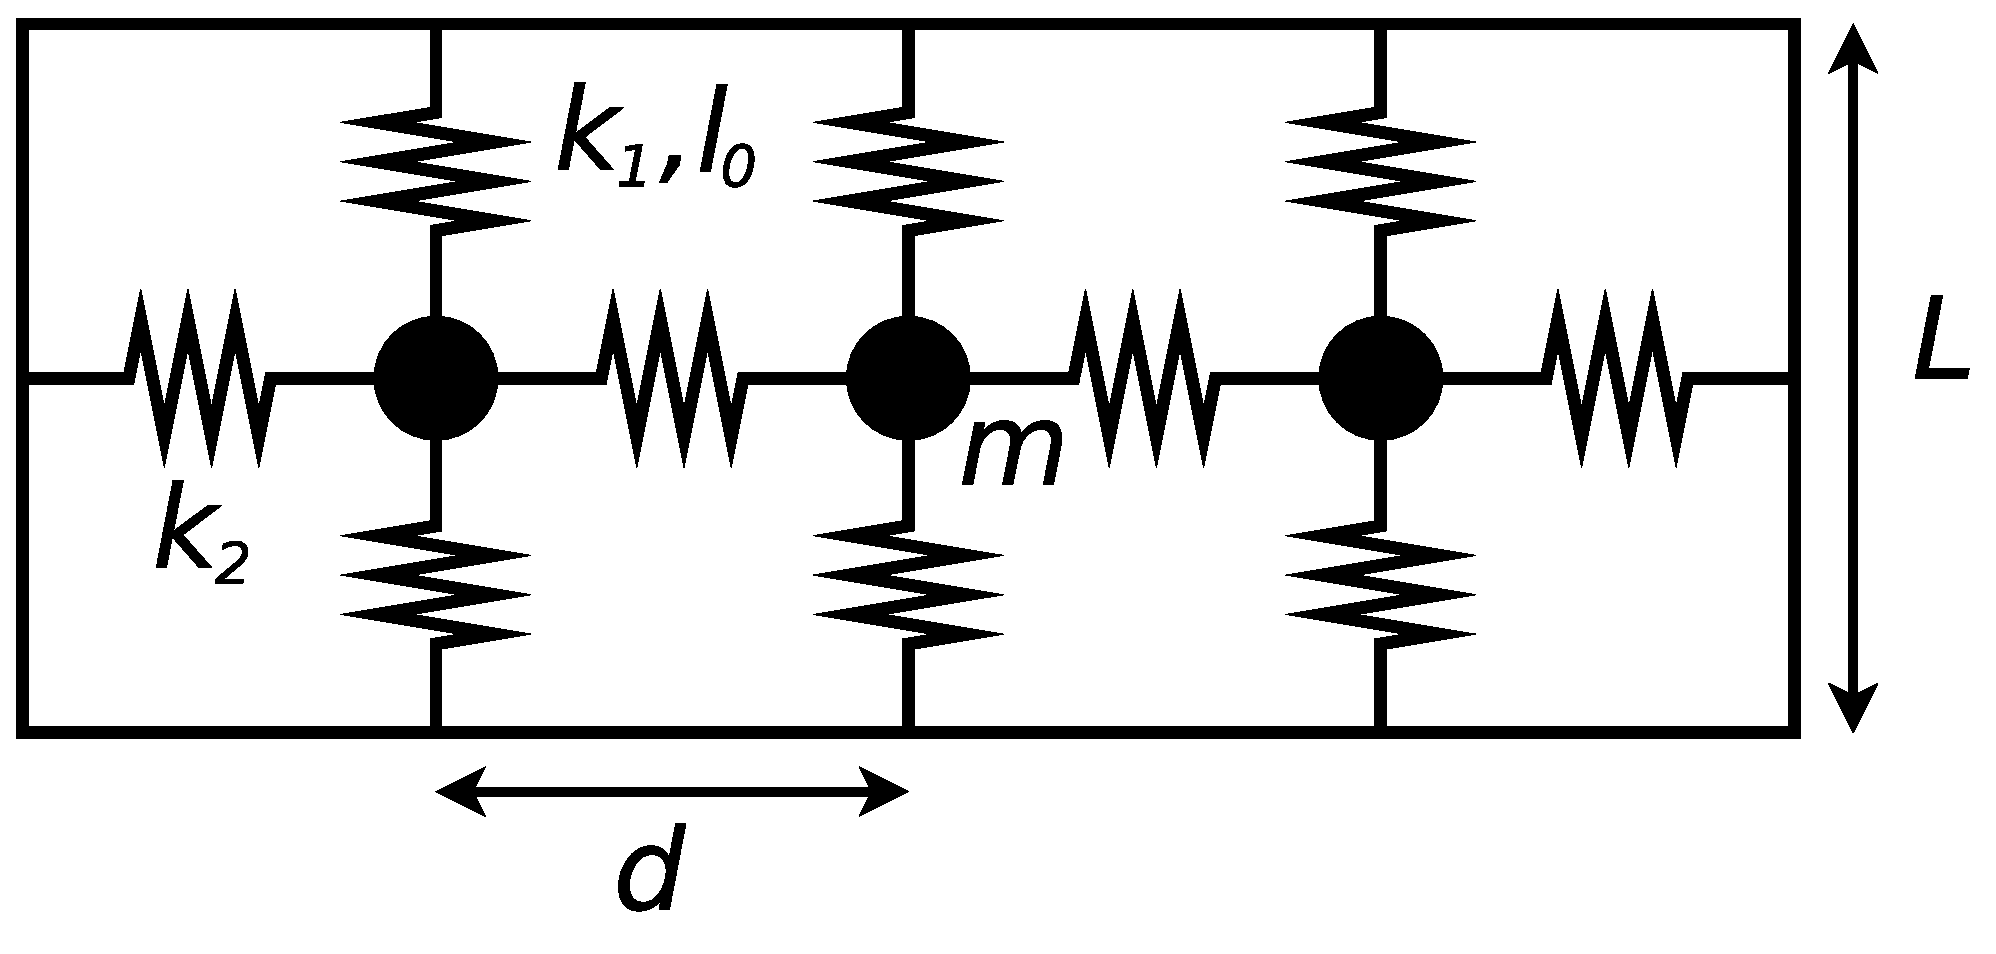
\includegraphics[width=\textwidth]{ej1-10}
\end{minipage}
